\documentclass[tikz,border=3pt]{standalone}
\usepackage[T1]{fontenc}
\usepackage{lmodern}
\usepackage{pgfplots,pgfplotstable}
\pgfplotsset{compat=1.18}
\definecolor{DukeBlue}{HTML}{00539B}
\definecolor{Navy}{HTML}{012169}
\definecolor{Teal}{HTML}{247F83}
\definecolor{Gold}{HTML}{B3853A}
\pgfplotsset{every axis/.append style={font=\sffamily\small,axis line style={black!35},tick style={black!35},grid style={black!8},axis x line*=bottom,axis y line*=left}}
\begin{document}
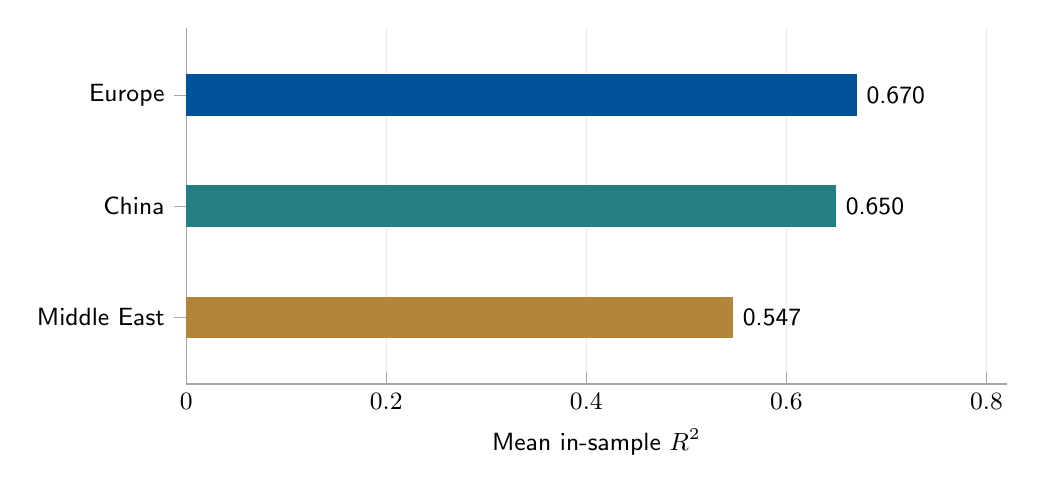
\begin{tikzpicture}
\begin{axis}[width=12cm,height=6.1cm,xbar,bar width=15pt,
 xmin=0,xmax=0.82,xtick={0,0.2,0.4,0.6,0.8},xlabel={Mean in-sample $R^2$},
 ytick={0,1,2},yticklabels={Europe,China,Middle East},y dir=reverse,
 ymin=-0.6,ymax=2.6,xmajorgrids,nodes near coords,nodes near coords style={font=\sffamily\small,anchor=west},point meta=explicit symbolic]
\addplot[fill=DukeBlue,draw=none,bar shift=0pt] coordinates {(0.670335,0) [0.670]};
\addplot[fill=Teal,draw=none,bar shift=0pt] coordinates {(0.649560,1) [0.650]};
\addplot[fill=Gold,draw=none,bar shift=0pt] coordinates {(0.546741,2) [0.547]};
\end{axis}
\end{tikzpicture}
\end{document}
